\documentclass{beamer}
\usepackage[OT1]{fontenc}
\usepackage[utf8]{inputenc}
%\setmainfont{STIX}
%\usepackage{unicode-math}
%\setmathfont{STIX Math}

\usepackage[british]{babel}

\usepackage[export]{adjustbox}

%\usepackage{cite}
\usepackage{graphicx}
\usepackage{amsmath}
\usepackage{caption}

\usepackage{multirow}

\usepackage{mathtools}
\usepackage{bm}
\usepackage{textcomp}
\let\v\bm
\def\mat#1{\bm{#1}}
\def\mul{\cdot}

\usepackage{siunitx}

\usepackage[linesnumbered,ruled]{algorithm2e}
\newcommand{\KwAssign}{\ensuremath{\leftarrow}}

\usepackage{url}

\title{Biotech Beer Brewing}
\subtitle{Or: How I Learned to Stop Worrying and Control the Lactobacilli}
\author{Dominik Schmidt, ETH Zürich\\Jakob Wittman, TU München}
\institute{Háskóli Íslands}
\date{\today}
\titlegraphic{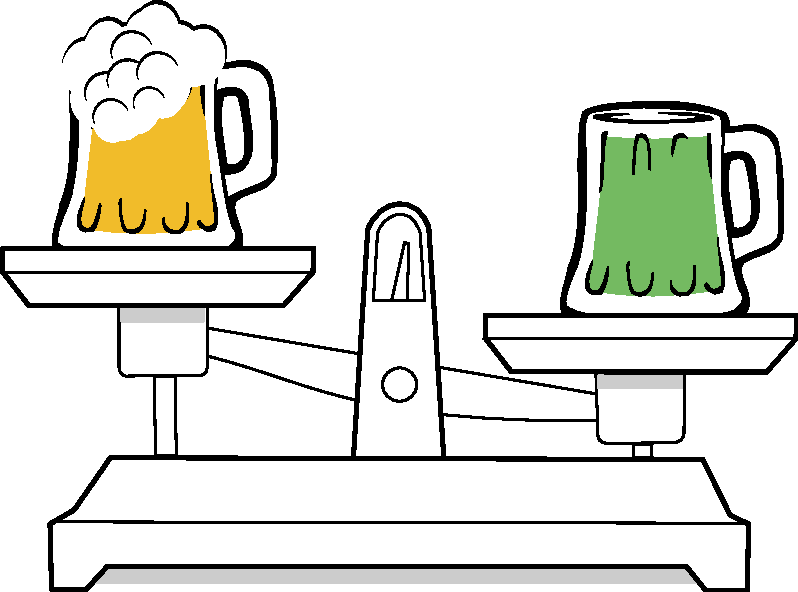
\includegraphics[width=0.3\linewidth]{../Graph/Logo.pdf}}
\logo{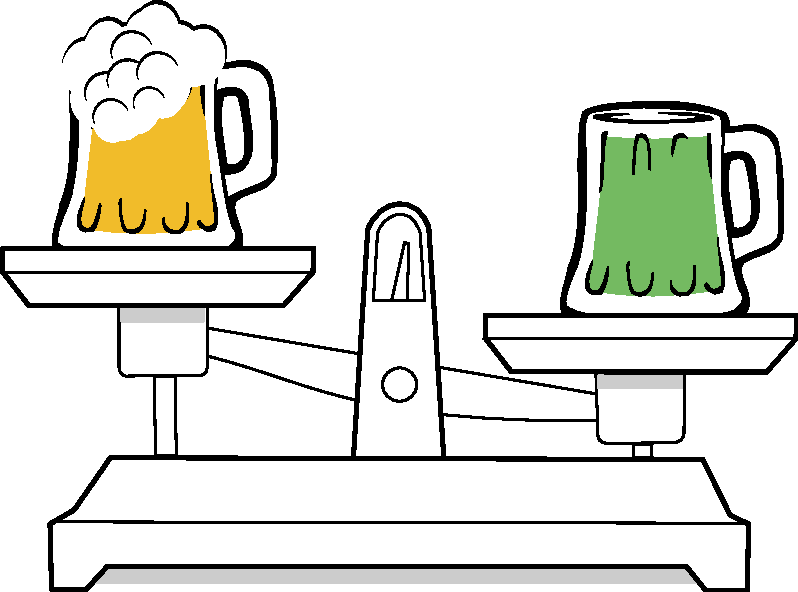
\includegraphics[width=5em]{../Graph/Logo.pdf}}
\beamertemplatenavigationsymbolsempty

\usepackage{xcolor}
\usepackage{tikz}
\usetikzlibrary{calc}
\usetikzlibrary{arrows}
\usetikzlibrary{positioning}

\begin{document}
\begin{frame}[plain]
	\titlepage
\end{frame}
\begin{frame}
  \frametitle{Content}
  \tableofcontents
\end{frame}

\section{Introduction}
\begin{frame}{Introduction}
  \begin{block}{Contamination in alcoholic fermentation}
    \begin{itemize}
      \item Bacterial contamination lowers the productivity of yeast (up to 30\% loss)
      \item mostly Lactobacillus plantarum and wild yeasts
      \item high quality standards in food industry (beer, wine, whisky,...)
    \end{itemize}
  \end{block}

  \begin{block}{How find process optimizations?}
    \begin{itemize}
     \item experiments with real cultures are expensive and time consuming
     \item simulation methods using genome-scale models gaining popularity
    \end{itemize}
  \end{block}
\end{frame}

\begin{frame}{Material}{Overview}

\begin{figure}[!h]
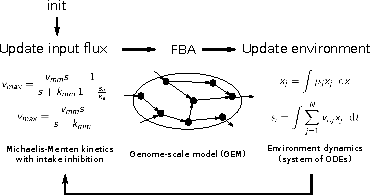
\includegraphics[width=\linewidth]{Img/dfba.pdf}
\caption{Dynamic flux balance analysis iteration step}
\label{fig:dfba}
\end{figure}
\end{frame}

\section{Material}
\begin{frame}{Material}{Tools}
    \begin{itemize}
      \item python 3
      \item dopri5 ODE solver, scipy.integrate.ode package \cite{hairer1993solving}
      \item COBRApy package \cite{heirendt_creation_nodate}
      \item \textit{Dynamic Multispecies Metabolic Modeling} (DMMM) framework (Matlab)\cite{zhuang_design_2012}
    \end{itemize}
\end{frame}

\begin{frame}{Material}{Simulation setup}
	\begin{minipage}{0.5\linewidth}
	\begin{itemize}
		\item Lactobacillus Plantarum (iBT721) $\leftrightarrow$ Saccharomyces Cerevisiae (iFF708)
		\item Consider monocultures first
		\item Compare monocultures with known outcomes
		\item Tweak paramteres if necessary (some parameters are not well known)
		\item Inspect the coculture
	\end{itemize}
	\end{minipage}
	\hfill
	\begin{minipage}{0.45\linewidth}
		\begin{figure}
			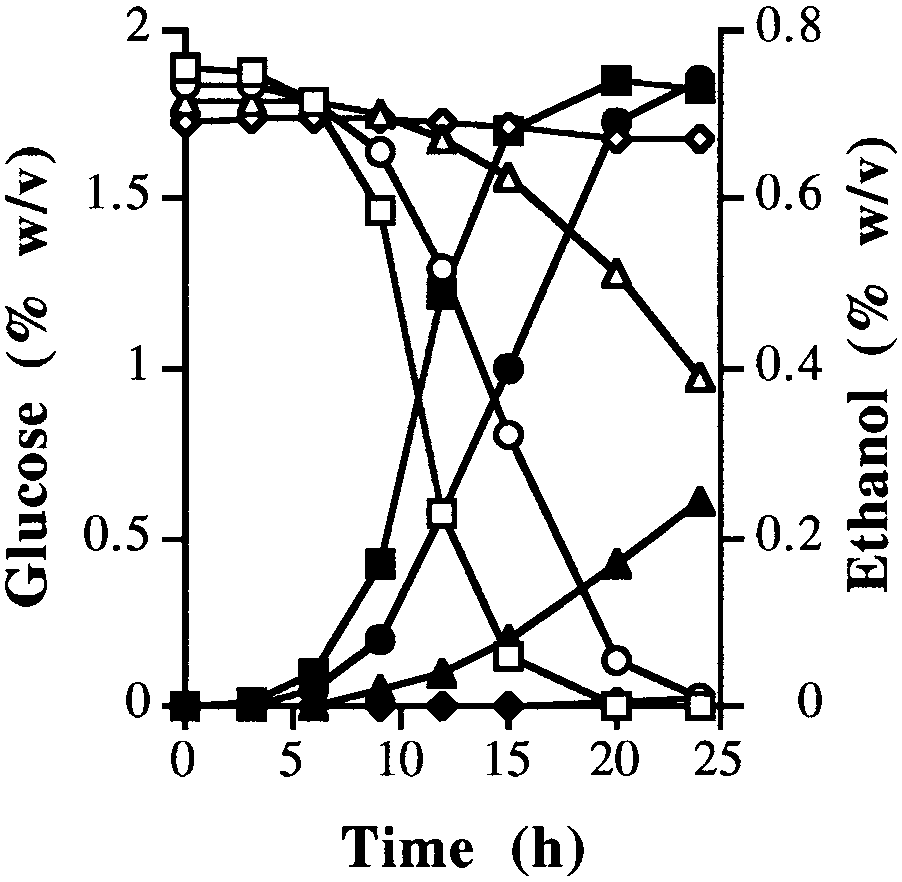
\includegraphics[width=0.8\linewidth]{Img/yeast_real.png}
			\caption{Known glucose and ethanol curves for yeast from \cite{narendranath_effects_1997}}
		\end{figure}
	\end{minipage}
\end{frame}

\section{Results}

\begin{frame}{Yeast Monoculture}{Population}
	\begin{figure}
		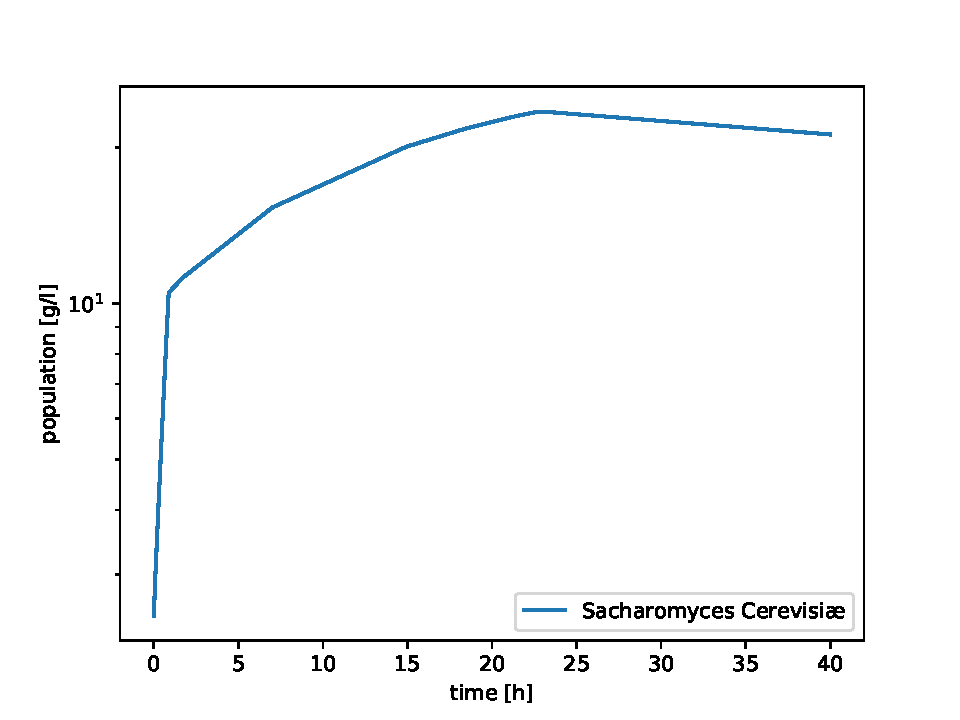
\includegraphics[width=0.9\linewidth]{Img/Results/yeast/0lac_populations.pdf}
	\end{figure}
\end{frame}

\begin{frame}{Yeast Monoculture}{Metabolites}
	\begin{figure}
		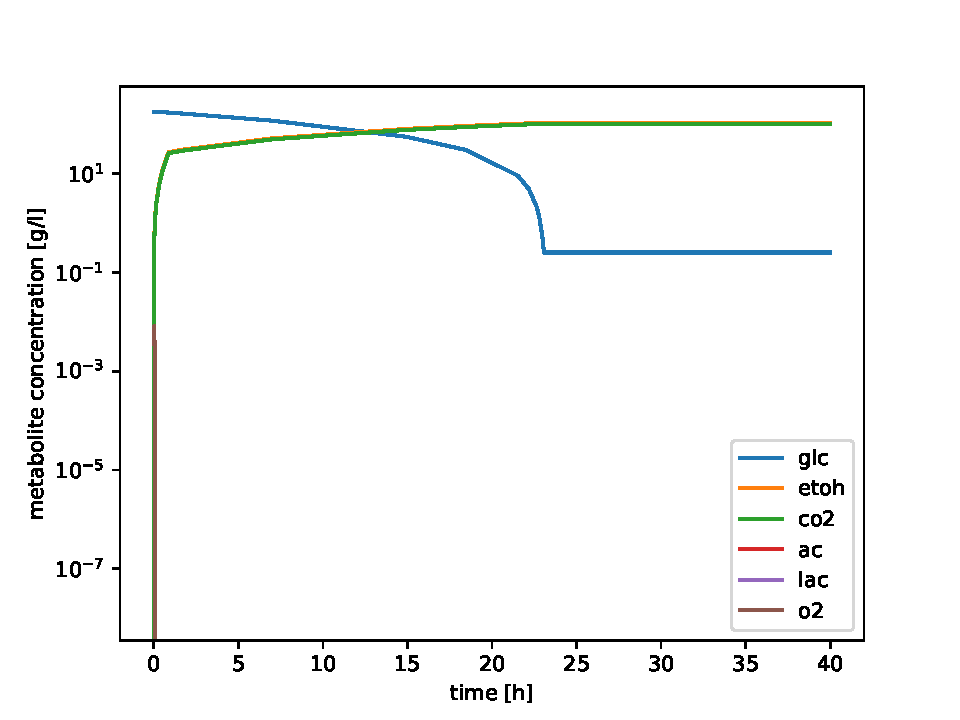
\includegraphics[width=0.9\linewidth]{Img/Results/yeast/0lac_metabolites.pdf}
	\end{figure}
\end{frame}

\begin{frame}{Lactobacillus Monoculture}{Population}
	\begin{figure}
		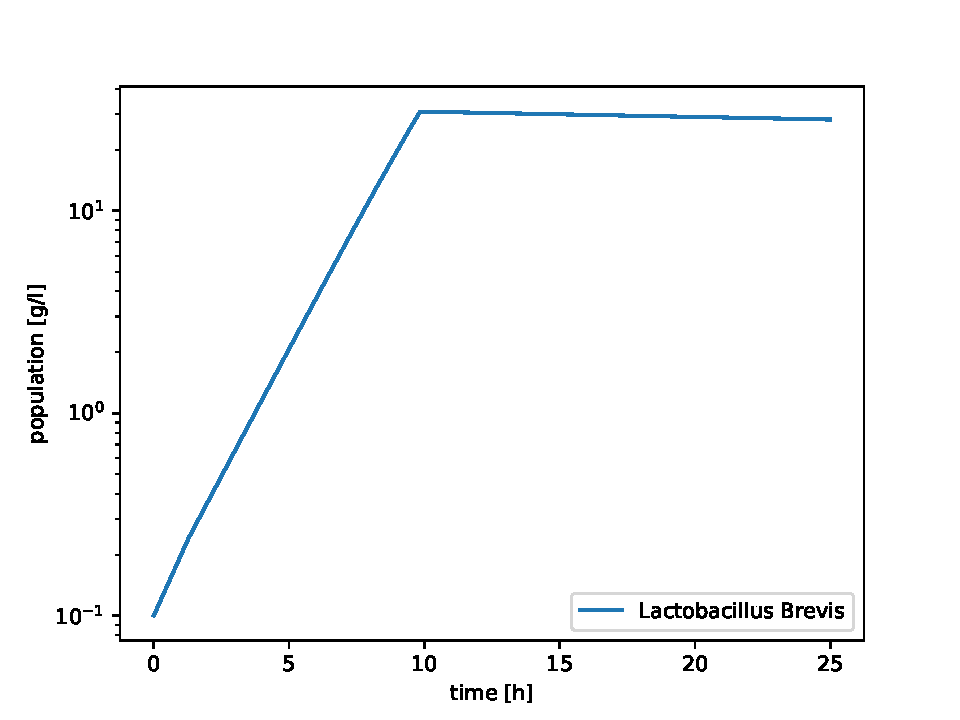
\includegraphics[width=0.9\linewidth]{Img/Results/lactobacillus/lactobacillus_populations.pdf}
	\end{figure}
\end{frame}

\begin{frame}{Lactobacillus Monoculture}{Metabolites}
	\begin{figure}
		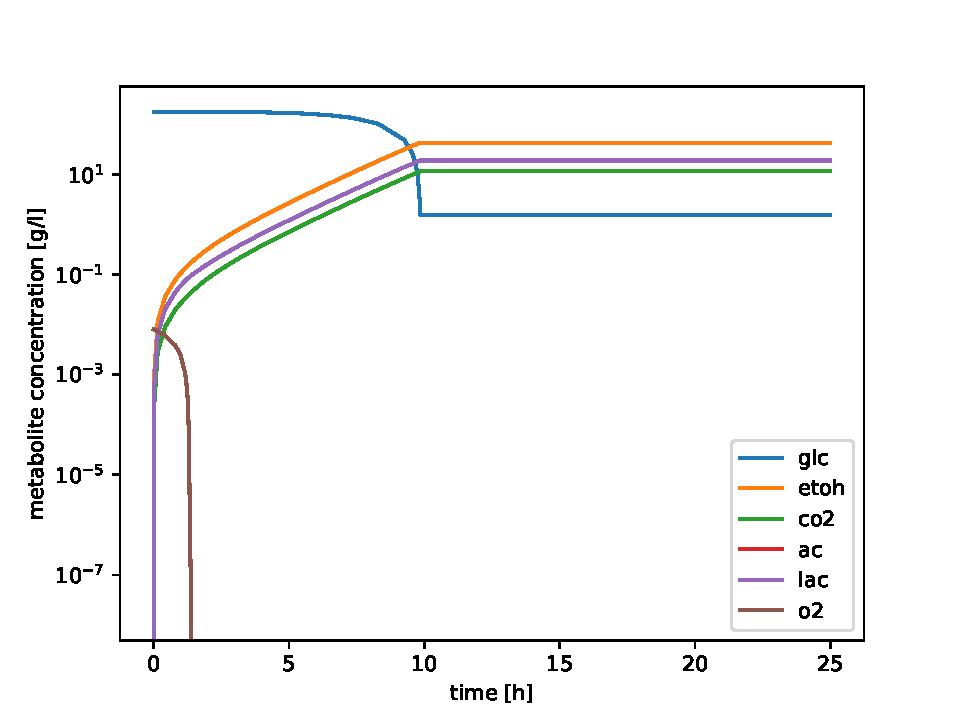
\includegraphics[width=0.9\linewidth]{Img/Results/lactobacillus/lactobacillus_metabolites.pdf}
	\end{figure}
\end{frame}

\begin{frame}{Coculture}{Population}
	\begin{figure}
		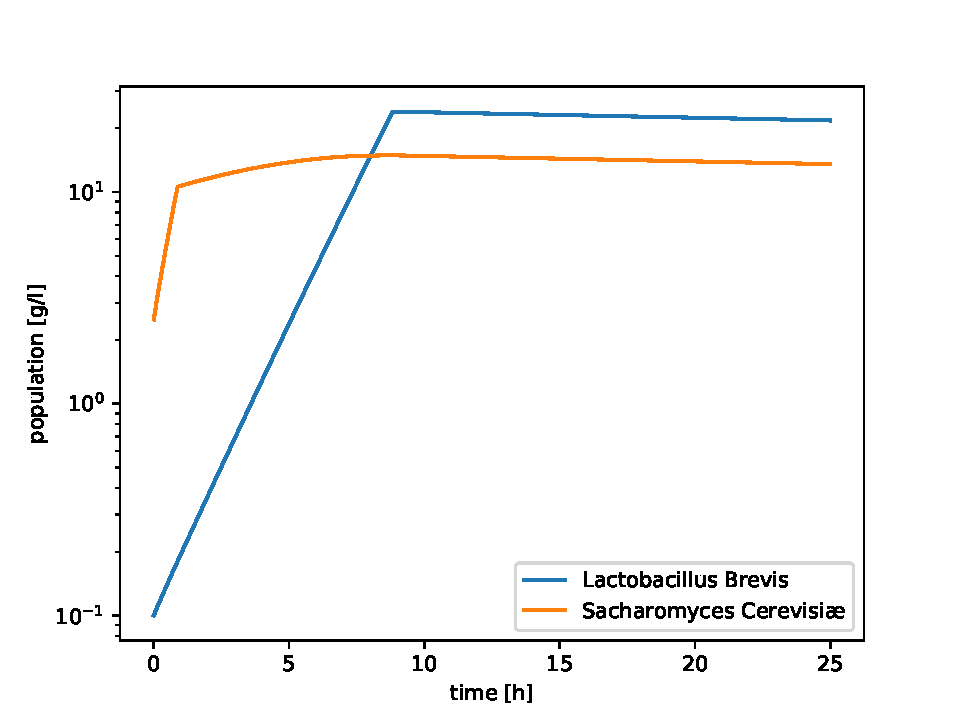
\includegraphics[width=0.9\linewidth]{Img/Results/cocultures/cocult2_populations.pdf}
	\end{figure}
\end{frame}

\begin{frame}{Coculture}{Metabolites}
	\begin{figure}
		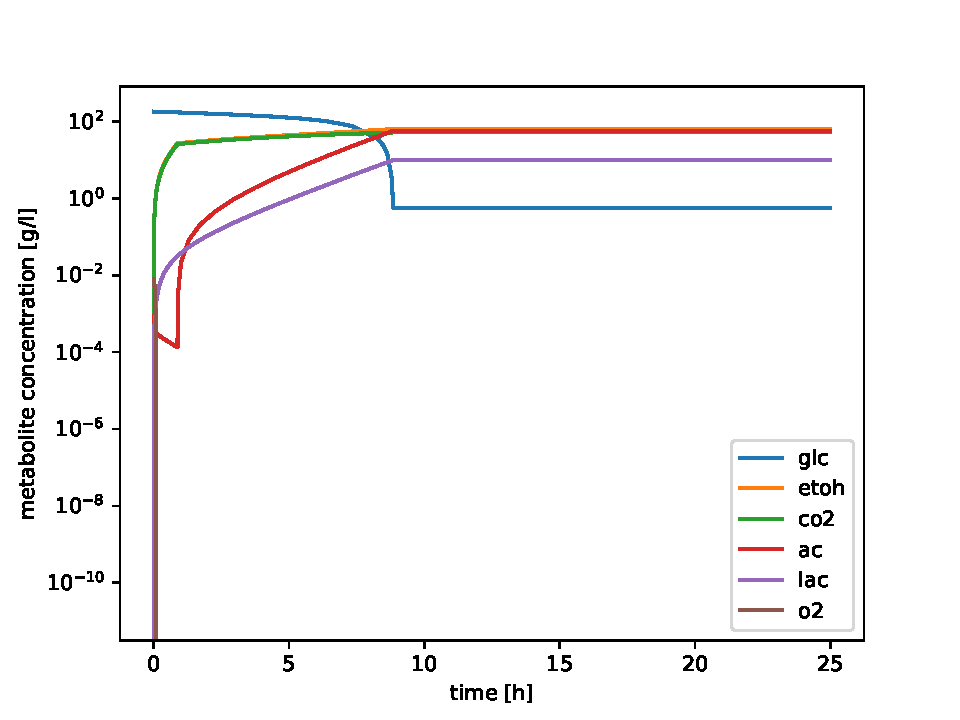
\includegraphics[width=0.9\linewidth]{Img/Results/cocultures/cocult2_metabolites.pdf}
	\end{figure}
\end{frame}

\section{Conclusions and next steps}
\begin{frame}
	\begin{itemize}
		\item Implement metabolite exchange with environment
		\item Recycle dead cells via "reverse biomass function"
		\item Alter the initial medium to be "harsher"
		\item More research on the co-culture
		\item More research on other co-cultures
		\item More research on taste and effect of beer (for science)
	\end{itemize}
\end{frame}

\appendix
\section<presentation>*{\appendixname}
\subsection<presentation>*{For Further Reading}
\begin{frame}[allowframebreaks]
  \frametitle{References}
  
  \bibliographystyle{IEEEtran}
  \bibliography{./../final_report/references}
\end{frame}
\end{document}
